\chapter{The D-Wave Quantum Computer}


TODO: intro del capítulo


\section{Quantum Annealing}


Simulated annealing (SA) is an general optimization technique that was first introduced in 1983 by Kirkpatrick \emph{et al.} \cite{Kirkpatrick1983}. The main idea is to mimic how thermal fluctuations work to let the system escape from local minimums in the cost function. The \emph{temperature} of the system dictates the probability with which the is allowed to jump to worse solutions (higher values of the cost function). The \emph{annealing schedule} is the decrease rate of the temperature, controlled by the programmer. Under the appropiate one, the system would be able to scape from local minimums to reach the global one. If the temperature decreases too quickly, the system converges prematurely to a local minimum. If it decreases too slowly, the technique transforms into a random walker, reaching the global minimum at some point but being worthless time-wise.

Inspiration in thermal fluctuations are used in SA so the system may escape from local minima. Similarly, \emph{quantum tunneling} is used in Quantum Annealing (QA) in order to escape from local minimums. This new technique was introduced in its present form by two similar proposals \cite{Finnila1994} \cite{Kadowaki1998}.

Quantum tunneling is a quantum mechanical phenomenon where a wavefunction (i.e. a quantum state) may propagate through a potetial barrier \cite{Nimtz2008}. The probability of this event occuring depends on the height and width of the barrier (see figure \ref{fig 2.1})

\begin{figure}[h]
	\includegraphics[scale=.8]{QuantumTunneling.jpg}
	\centering
	\caption{Thermal jumps vs quantum tunneling.}
	\label{fig 2.1}
\end{figure}

The main advantage of quantum tunneling compared to classical thermal fluctuations is that the probability of the system shifting depends to only on the height of the potential barrier but also on its width. Thus, application of QA may pottentially outperform SA in problems where the energy (cost) landscape consists on very high and thin barries surronding local minimums. 

Particularly, as studied in \cite{Ray1989}, let $\Delta$ be the height of a barrier and $\omega$ its width. The probability of a thermal transition ocurring is dictated by $exp\{-\frac{\Delta}{k_B T}\}$ where $T$ y the temperatue of the system and $k_B$ is the Boltzmann constant. On the other hand, the probability of a quantum tunneling transition ocurring through the same barrier (asumming isolation) is $exp\{-\frac{\sqrt \Delta \omega}{\Gamma}\}$, where $\Gamma$ is the tunneling field. Thus, the probability is much higher for the quantum tunneling effect on a high and thin barriers.

We may also observe looking at the previous expressions how the tunneling field and the temperature play a similar roles in the different methods. Thus, the annealing schedule of the QA system is controlled using the tunneling field just like the temperature is used in SA.

There are many examples in the literature of QA simulations using classical computers, both theoretical \cite{Morita2008} and numerical -most of them using Quantum Monte Carlo (QMC) methods \cite{Isakov2016} \cite{Farhi2000}-. This evidence suggests outperformance of SA by simulated QA under certain conditions. It is resonable to wonder what happens if instead of simulating QA we could somehow encode our problems in a real physical system that tends to its lower energy state (ground state), thus using quantum tunneling naturally. This is precisely what the D-Wave system does.

In section \ref{quantum-annealing-dwave} we will depeen in the technicalities of quantum annealing, how it is implemented and how to use in the D-Wave system.


\section{QUBO and Ising problems}





TODO: completar sección





\section{D-Wave Systems}


\textbf{D-Wave Systems Inc.} is a Canadian company dedicated to quantum computing. In 2011, they announced the first commercial quantum computer system, D-Wave One. During the following two decades, the D-Wave team have developed a series of computing computers dedicated to quantum annealing. The last one being the Advantage System (figure \ref{fig 2.2}).

\begin{figure}[h]
	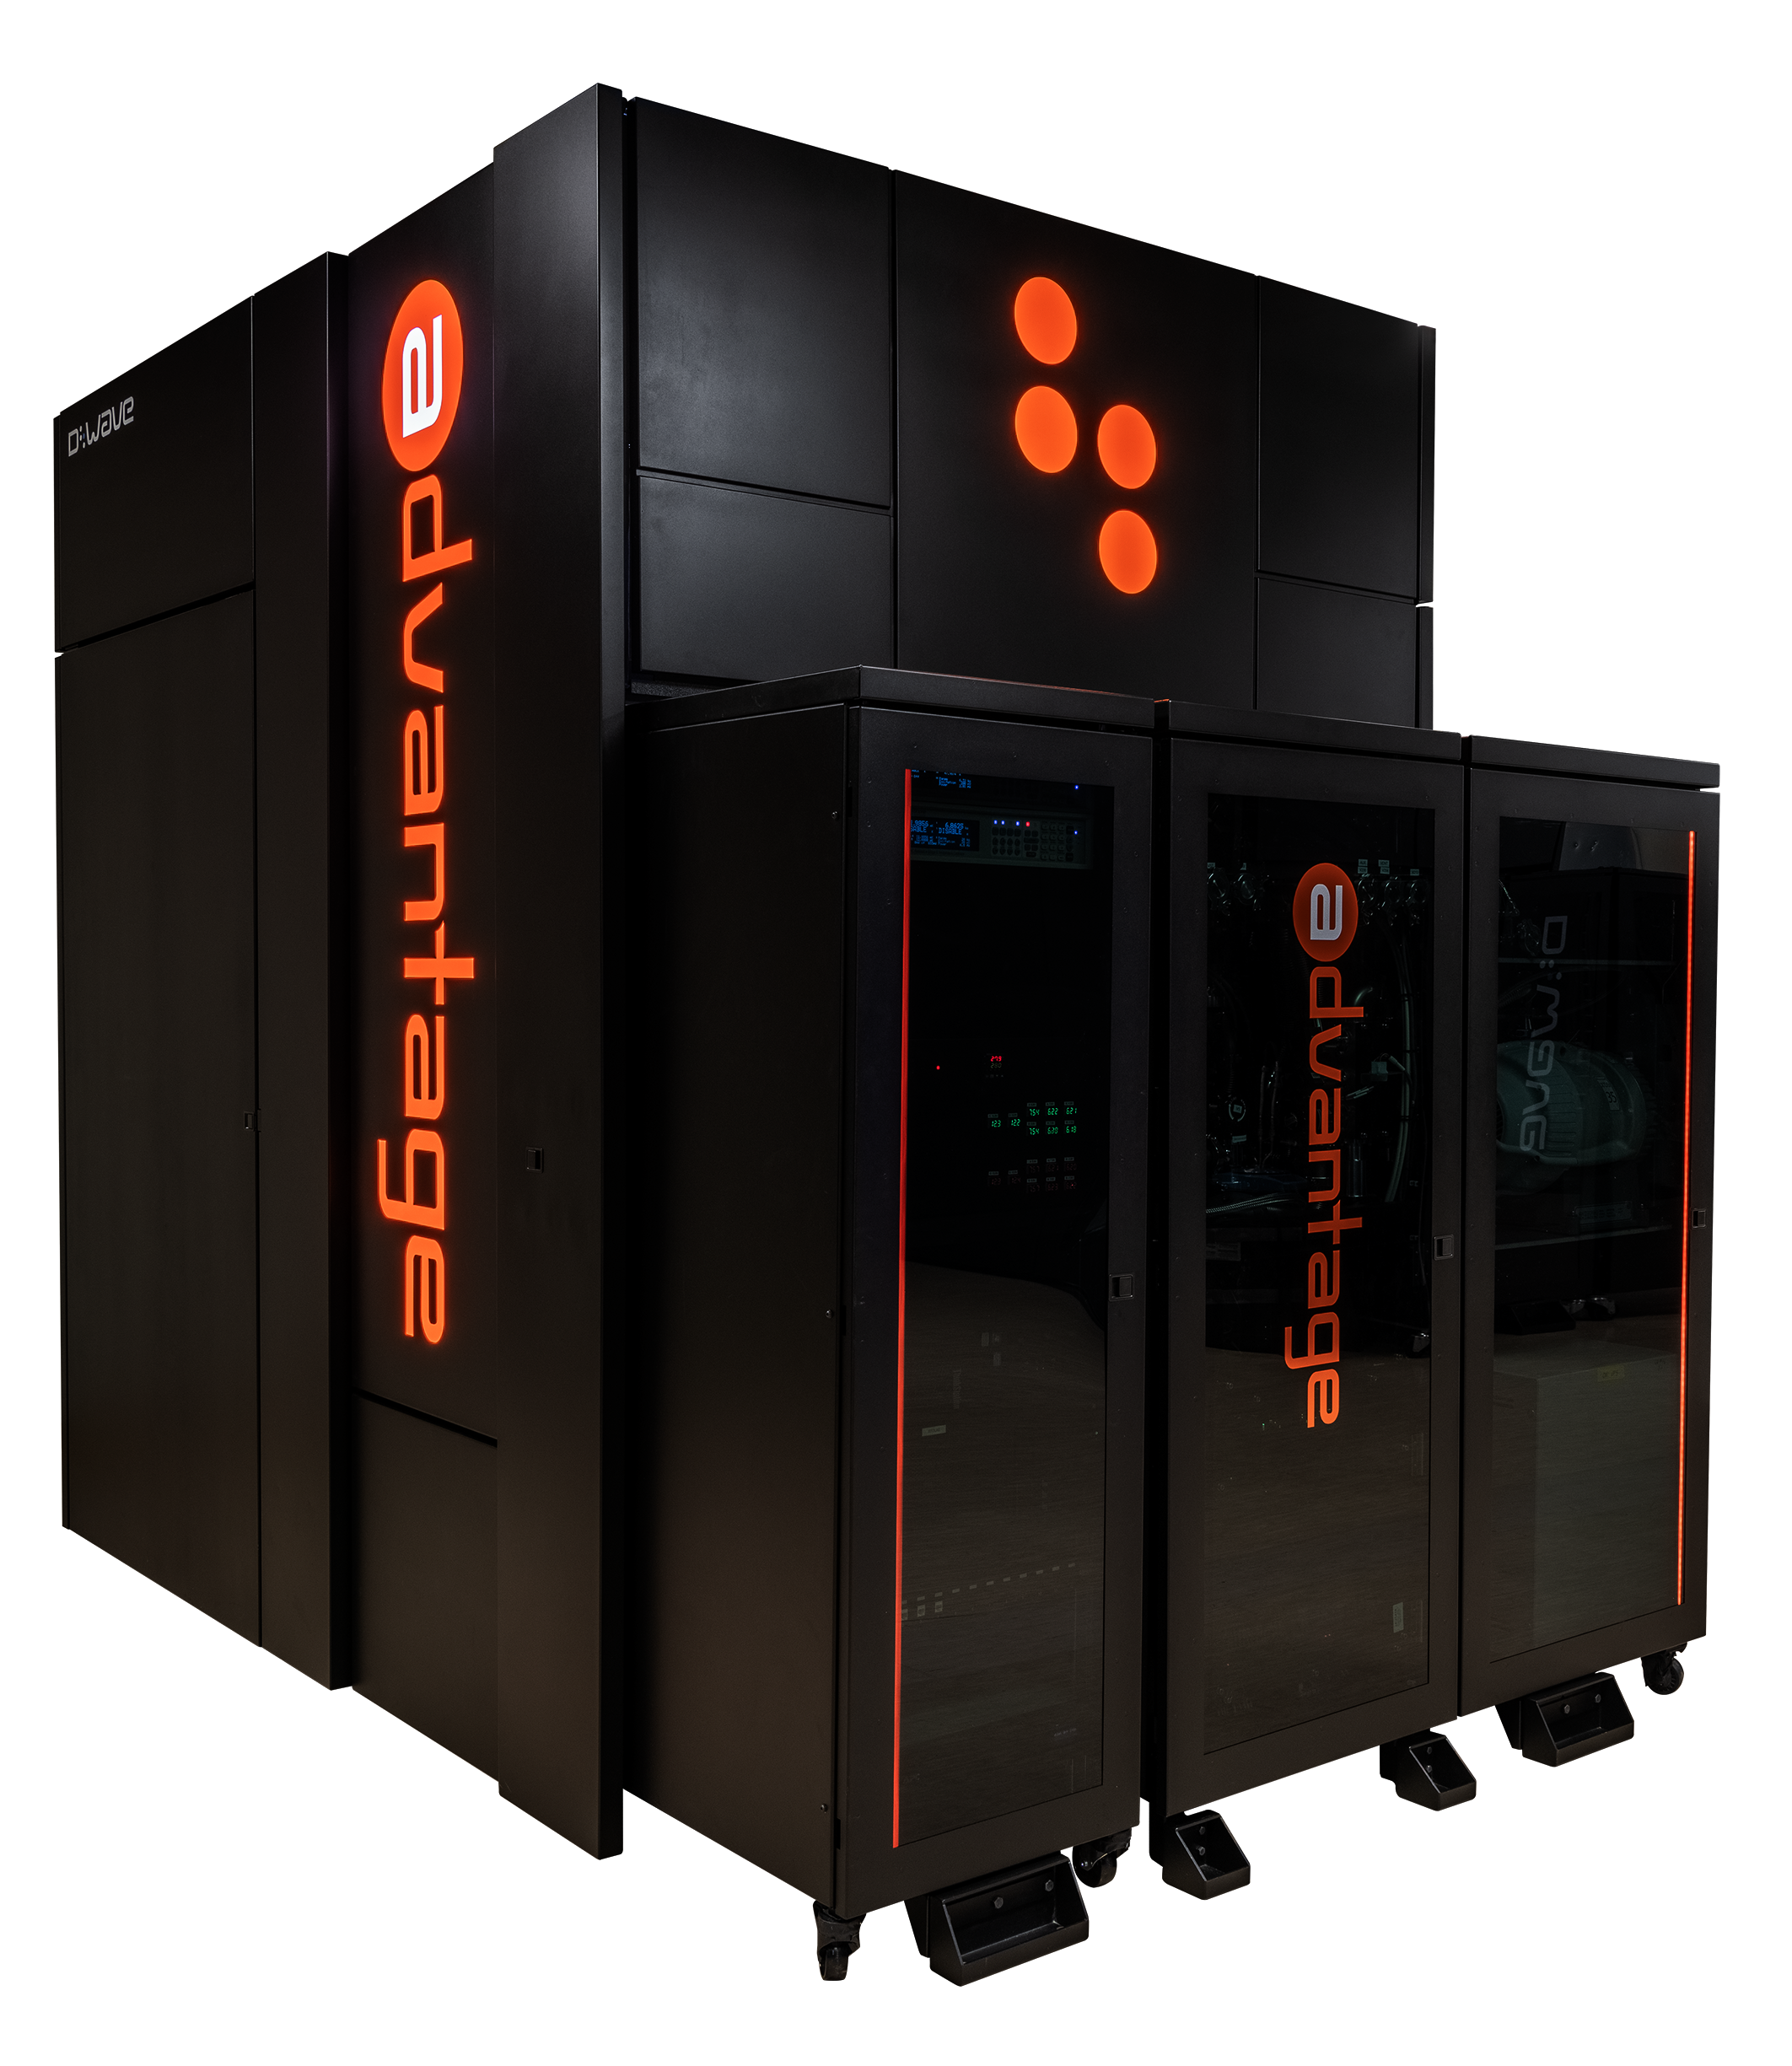
\includegraphics[scale=.1]{advantage_system.png}
	\centering
	\caption{Advantage$^{TM}$ system}.
	\label{fig 2.2}
\end{figure}

The quantum processing unit (QPU) of this system consist of $5640$ qubits and $40,484$ \emph{couplers} (links between qubits that allow entanglement between a pair of qubits). The number of couplers is especially relevant. It tells us that not every qubit can be entangled with every other qubit. We will come back to this in section [TODOref]. Since the QPU must be isolated to operate, it is encapsulated in a system at temperatures below 15 mK. In addition, radio frequency (RF)-shielded enclousre and magnetic shieldings are used to protect it from electromagnetic interferience \cite{DWaveDoc}.

\begin{figure}[h]
	\includegraphics[scale=.2]{qpu.png}
	\centering
	\caption{D-Wave QPU}.
	\label{fig 2.3}
\end{figure}

D-Wave provides an easy-to-use software enviroment to solve problems using quantum annealing. We will explain in depth in section [TODOref].


\subsection{Quantum Annealing in D-Wave}
\label{quantum-annealing-dwave}


For this section we refer to the D-Wave documentation, which explains how quantum annealing is implemented and may be exploited in the D-Wave systems \cite{DWaveDoc-QuantumAnnealing}.




TODO: rephrasear la cita en el contexto anterior











https://journals.aps.org/prl/pdf/10.1103/PhysRevLett.117.180402




